\documentclass{book}
\usepackage[a4paper,top=2.0cm,bottom=2.0cm,left=2.0cm,right=3.0cm]{geometry}

%\documentclass[pdftex,10pt,a4paper]{book}
%\usepackage[paperwidth=19cm,
%paperheight=26cm, outer=2cm, 
%top=1.5cm, bottom=1.5cm]{ geometry}

\usepackage[english,italian]{babel} %l'ultima lingua è quella che legge per i titoli
\usepackage[utf8]{inputenc}
\usepackage[T1]{fontenc,url}
\usepackage{titlesec}
\usepackage{easylist}
\usepackage{hanging}

\usepackage[pdftex,colorlinks]{hyperref}
\hypersetup{
	colorlinks=true,
	linkcolor=black,
	filecolor=magenta,
	urlcolor=cyan,
}
\usepackage{hypcap}
\usepackage{blindtext}
\usepackage{tipa}
\usepackage{epigraph}
\usepackage{enumerate}
\usepackage{longtable}
\usepackage{setspace}
\usepackage{verbatim}
\usepackage{graphicx}
\usepackage{amsmath}
\usepackage{pbox}
\usepackage{fancyhdr}
\usepackage{cancel}
\usepackage{tabularx}
\usepackage{booktabs}
\usepackage{multirow}
\usepackage{longtable}
\usepackage{tikz}
\usepackage{tikz-qtree}
\usepackage{subfig}
\usepackage{xcolor}
\usepackage{amssymb}
\usepackage{amsmath}
\usepackage{mathrsfs}
\usepackage{textcomp}
\usepackage{circuitikz}
\usepackage{pifont}
\usepackage{imakeidx}
\usepackage{verbatim}
\usepackage{dsfont}
\usepackage{listings}
\usepackage{color}
\usepackage{upgreek}
\usepackage{tasks}
\usepackage{exsheets}
\usepackage{pgfplots}
\usepackage{amsthm}
\usepackage{wasysym}
\usepackage{qtree}

\usepackage{showframe}
\renewcommand\ShowFrameLinethickness{0.15pt}
%\renewcommand*\ShowFrameColor{\color{red}}

%\usepackage{showkeys} %serve per mostrare le etichette "tag" o target, va tolta per la versione definitiva;

\SetupExSheets[question]{type=exam}

\definecolor{mygreen}{rgb}{0,0.6,0}
\definecolor{mygray}{rgb}{0.5,0.5,0.5}
\definecolor{mymauve}{rgb}{0.58,0,0.82}

\lstset{ 
  backgroundcolor=\color{white},   % choose the background color; you must add \usepackage{color} or \usepackage{xcolor}; should come as last argument
  basicstyle=\footnotesize,        % the size of the fonts that are used for the code
  breakatwhitespace=false,         % sets if automatic breaks should only happen at whitespace
  breaklines=true,                 % sets automatic line breaking
  captionpos=b,                    % sets the caption-position to bottom
  commentstyle=\color{mygreen},    % comment style
  deletekeywords={...},            % if you want to delete keywords from the given language
  escapeinside={\%*}{*)},          % if you want to add LaTeX within your code
  extendedchars=true,              % lets you use non-ASCII characters; for 8-bits encodings only, does not work with UTF-8
  firstnumber=1000,                % start line enumeration with line 1000
  frame=single,	                   % adds a frame around the code
  keepspaces=true,                 % keeps spaces in text, useful for keeping indentation of code (possibly needs columns=flexible)
  keywordstyle=\color{blue},       % keyword style
  language=Octave,                 % the language of the code
  morekeywords={*,...},            % if you want to add more keywords to the set
  numbers=left,                    % where to put the line-numbers; possible values are (none, left, right)
  numbersep=5pt,                   % how far the line-numbers are from the code
  numberstyle=\tiny\color{mygray}, % the style that is used for the line-numbers
  rulecolor=\color{black},         % if not set, the frame-color may be changed on line-breaks within not-black text (e.g. comments (green here))
  showspaces=false,                % show spaces everywhere adding particular underscores; it overrides 'showstringspaces'
  showstringspaces=false,          % underline spaces within strings only
  showtabs=false,                  % show tabs within strings adding particular underscores
  stepnumber=2,                    % the step between two line-numbers. If it's 1, each line will be numbered
  stringstyle=\color{mymauve},     % string literal style
  tabsize=2,	                   % sets default tabsize to 2 spaces
  title=\lstname                   % show the filename of files included with \lstinputlisting; also try caption instead of title
}

\frenchspacing

\newcommand{\abs}[1]{\lvert#1\rvert}

\usepackage{floatflt,epsfig}

\usepackage{multicol}
\newcommand\yellowbigsqcup[1][\displaystyle]{%
  \fboxrule0pt
  \ifx#1\textstyle\fboxsep-0.6pt\else\fboxsep-1.25pt\fi
  \mathrel{\fcolorbox{white}{yellow}{$#1\bigsqcup$}}}
% definizioni
\newtheorem{esercizio}{Esercizio}[section]
\newtheorem{teorema}{Teorema}[section]
\newtheorem{nota}{Nota}[section]
\theoremstyle{definition}
\newtheorem{defi}{Definizione}[section]
\newtheorem{esempio}{Esempio}[section]
\newtheorem{svol}{Svolgimento}[section]
\newtheorem{oss}{Osservazione}[section]

\title{reti di telecominicazione}
\author{Nicola Ferru}
\begin{document}
\begin{titlepage}
%	\tikz[remember picture,overlay] \node[opacity=0.50,inner sep=0pt, scale=0.8] at (current page.center){\includegraphics[width=\paperwidth,height=\paperheight]{./backround/backround.png}};
	\begin{center}
		
		% Upper part of the page
		\includegraphics[scale=.45]{./title/logo_CA.jpg}
		\\
		\vspace{1cm}
		\textsc{\large Università degli Studi di Cagliari}
		\vspace{1.2cm}
		
		\textsc{\Large DIEE}
		\vspace{0.5cm}
		
		\textsc{\large Dipartimento di Ingegneria e Architettura}
		\vspace{1.0cm}
		
		\textsc{\large Corso di Laurea {Triennale} in Ingegneria Elettrica industriale}\hspace{0.8cm}
		
		% Title
		\vspace{0.8cm}
		
		\Huge \doublespacing \bfseries \begin{spacing}{1}{ANALISI MATEMATICA 2}\end{spacing}
		\hfill
		\normalsize \itshape \begin{spacing}{1}{}\end{spacing}
		\hfill
		\normalsize\itshape \begin{spacing}{1}{edited by}\end{spacing}
		\hfill
		\Large\itshape  \begin{spacing}{1}{NICOLA FERRU}\end{spacing}
		\vspace{0.5cm}
		%		% Author and supervisor
		%		\begin{flushleft} \large
			%			\emph{Relatore:} \\
			%			Ch.mo Prof. Nome \textsc{Cognome}
			%		\end{flushleft}
		%		\vfill
		%		\begin{flushright} \large
			%			\emph{Laureando:}\\
			%			Nome \textsc{Cognome}
			%			
			%			\textsc{Matricola N. 1234567}
			%		\end{flushright}
		
		\hfill
		\vfill
		\Large \bfseries \begin{spacing}{1}{Unofficial Version}\end{spacing}
		\vspace{0.5cm}
		% Bottom of the page
		%{\small 4 Ottobre 2018 -  \today{}}
		{\small 2022 -  2023}
	\end{center}
	\clearpage
	\thispagestyle{empty}
	\vspace*{\fill}%
	{\centering [This page is intentionally left blank]\par}%
	\vspace{\fill}
\end{titlepage}

\tableofcontents
\chapter{Introduzione}
\label{chap:intro}
\begin{defi}
  GNU/Octave è un applicativo per il calcolo matriciale che consente di svilgere
  tutte le operazioni base e non solo a riguardo, dallo somma, divisione,
  moltiplicazioni e sottrazioni tra matrici, calcolo del determinante, del
  grado e tanto altro.
\end{defi}

\section{Pacchetti e impostazioni base}
\label{sec:packbase}

\subsection{Pacchetti}
\label{sec:pack}

\begin{table}[th]
  \centering
  \begin{tabular}{ll}
    {\bf Nome} & {\bf Descrizione}\\\hline
    \href{https://gnu-octave.github.io/packages/fuzzy-logic-toolkit/}{fuzzy-logic-toolkit} & Un toolkit di logica fuzzy per lo più
                                                                                               compatibile con MATLAB per Octave \\\hline
    \href{https://gnu-octave.github.io/packages/symbolic/}{symbolic} & Aggiunge funzionalità di calcolo simbolico a GNU
                        Octave \\\hline
    \href{https://gnu-octave.github.io/packages/ocs/}{Circuit Simulator (OCS)} & Risolvere equazioni di circuiti elettrici DC e transitori. \\\hline
    \href{https://gnu-octave.github.io/packages/control/}{Control} & Strumenti CACSD ({\it Computer-Aided Control System
                       Design}) per GNU Octave,\\ &basati sulla libreria SLICOT.\\\hline
    \href{https://gnu-octave.github.io/packages/instrument-control/}{instrument-control} & Funzioni I/O di basso livello per interfacce seriali, i2c, parallele, tcp, gpib, vxi11,\\
               &udp e usbtmc.\\\hline 
  \end{tabular}
  \caption{pacchetti utili}
  \label{tab:pachutil}
\end{table}

\subsection{Funzione di identificazione di una variabile}
\label{sec:funiden}
\begin{table}[ht]
  \centering
  \begin{tabular}[tab:funzionediid]{ll}
    {\bf Nome} & {\bf Descrizione} \\\hline
    \lstinline|whos M| & stampa i dati completi sulla variabile
  \end{tabular}
  \caption{Funzione di identificazione}
  \label{tab:funzionediid}
\end{table}
\subsubsection{Stampa a video}
\label{sec:stampiden}
\begin{small}
\begin{verbatim}
Variables visible from the current scope:
variables in scope: top scope
  Attr   Name        Size                     Bytes  Class
  ====   ====        ====                     =====  =====
         M           3x3                         72  double
Total is 9 elements using 72 bytes
\end{verbatim}
\end{small}
\clearpage

\subsubsection{Come funziona}
All'interno di Octave e Matlab sono presenti le classi di variabili
esattamente come accade in altri linguaggi più di programmazione più blasonati,
esso ovviamente è relegato alle funzioni matematiche e grafiche per cui è
pensato il programma.
\begin{figure}[ht]
  \centering
  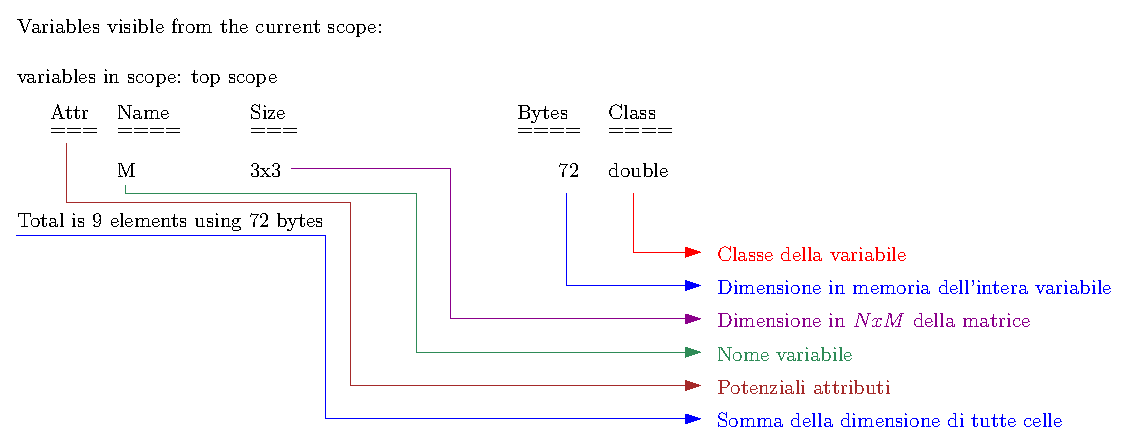
\includegraphics[width=15cm]{img/finiti/whos.eps}
  \caption{descrizione dell'interfaccia di funzione}
  \label{fig:interffun}
\end{figure}
\begin{notab}
  Anche la variabile singola viene vista come una matrice 1x1, da questo si
  denota che come il suo cugino Matlab è un software pensato per elaborare
  prodotti matriciali, infatti, il nome Matlab non sta per \texttt{Mathematic
    lab} ma per \texttt{Matrix Lab}. 
\end{notab}
\subsection{Tipi variabile}
\label{sec:tipivariabile}

\begin{table}[ht]
  \centering
  \begin{tabular}{llll}
    {\bf Nome} & {\bf Descrizione} & {\bf Dimensione} & {\bf Cifre rappresentabili}\\\hline
    \lstinline|double| ({\bf default}) & double-precision array & 8byte & $\pm1.79769x10^{308}$ a $\pm2.22507x10^{-308}$\\\hline
    \lstinline|single| & single-precision array & 4byte & $-2.1475x10^9$ a $2.1475x10^9$\\\hline 
    \lstinline|int8| & Array di interi con segno & 8bit & $-128$ a $127$\\\hline
    \lstinline|int16| & Array di interi con segno & 16bit & $-32768$ a $32767$ \\\hline
    \lstinline|int32| & Array di interi con segno & 32bit & $-2.1475x10^9$ a $2.1475x10^9$\\\hline 
    \lstinline|int64| & Array di interi con segno & 64bit & $-9.2234x10^{18}$ a $9.2234x10^{18}$\\\hline
    \lstinline|uint8| & Array di interi senza segno & 8bit & $255$\\\hline
    \lstinline|uint16| & Array di interi senza segno & 16bit & $65535$ \\\hline
    \lstinline|uint32| & Array di interi senza segno & 32bit & $4.2950x10^9$\\\hline 
    \lstinline|uint64| & Array di interi senza segno & 64bit & $1.8447x10^{19}$\\\hline
  \end{tabular}
  \caption{Tipi variabile}
  \label{tab:tipivariabile}
\end{table}
\begin{oss}
  Questa rapresentazione in memoria vale per la singola cella, quindi bisogna
  moltiplicare il paso per il numero di celle dello stesso tipo. Il programma
  peserà quanto il numero complessivo delle variabili presenti.
\end{oss}

\paragraph{Le stringhe --}
Un altro tipo di variabile però implicita sono le stringhe che il programma può
gestire, nel sequente modo \lstinline|str = "string x"| e la stampa di stringa
viene fatta con un semplice \lstinline|printf(str)|.
\clearpage
\subsubsection{Cosa stampa e cosa no}
Nel linguaggio di Matlab e Octave vengono stampate tutte le associazioni,
funzioni e inizializzazioni che non terminano con il ``{\color{red};}''.

\subsection{Impostazioni e formati}
\label{sec:formImp}
\begin{table}[ht]
  \centering
  \begin{tabular}{lll}
    {\bf Nome} & {\bf Descrizione} & {\bf Visuale}\\\hline
    \lstinline|rat| & Aspetto rateo (invece dei numeri reali rende numeri frazionari) & 1/2\\\hline
    \lstinline|short| & Formato breve a decimale fisso con 4 cifre dopo la virgola. (\textit{default}) & 0.5000\\\hline
    \lstinline|long| & Formato lungo a decimale fisso con 15 cifre dopo la virgola per & 0.500000000000000\\
                     &  i valori doppi e 7 cifre dopo la virgola per i valori singoli. \\\hline
    \lstinline|shortE| & Formato breve in annotazione scientiica con 4 cifre dopo la virgola & 5.0000e-01\\\hline
    \lstinline|longE| & Formato lungo a decimale fisso con 15 cifre dopo la virgola per & 5.000000000000000e-01\\
               & i valori doppi e 7 cifre dopo la virgola per i valori singoli.\\\hline
    \lstinline|shortG| & Formato breve, decimale fisso o notazione scientifica, a seconda & 0.5000\\
               & di quale sia più compatto, con un totale di 5 cifre.\\\hline
    \lstinline|longG| & Formato lungo a decimali fissi o notazione scientifica, qualunque & 0.500000000000000\\
               & sia il più compatto, con un totale di 15 cifre per i valori doppi e\\ & 7 cifre per i valori singoli.\\\hline
    \lstinline|shortEng| & Breve notazione ingegneristica (l'esponente è un
                           multiplo & 500.0000e-003\\
    
               &di 3) con 4 cifre dopo la virgola.\\\hline
    \lstinline|longEng| & Notazione ingegneristica lunga (l'esponente è un multiplo di 3) & 500.000000000000000e-003\\ & con 15 cifre significative.\\\hline
    \lstinline|+|&Formato positivo/negativo con caratteri +, - e vuoti visualizzati & +\\
               & per elementi positivi, negativi e zero.\\\hline
    bank & Formato valuta con 2 cifre dopo la virgola. & 0.50 \\\hline
    hex & Rappresentazione esadecimale di un numero binario & 3fe0000000000000 \\
               & a doppia precisione.\\\hline 
  \end{tabular}
  \caption{Impostazioni e formati}
  \label{tab:form}
\end{table}
\begin{notab}
  È possibile salvare il formato in una variabile con il comando \lstinline|fmt = format("nomeFormato")|
  per poi riutilizzarlo in seguito richiamando \lstinline|format(fmt)|. Altro aspetto esso può cambiare durante lo script quindi è possibile ripotare un dato
  in un formato di stampa e uno in un altro.
\end{notab}

\clearpage
\subsection{Flussi informativi}
\label{sec:flusinfo}

\begin{itemize}
\item Una entità è impegnata nella gestione di due flussi
\item Flusso con entità appartenenti agli strati adiacenti:
  \begin{itemize}
  \item Trasferimento diretto;
  \item Le \texttt{UI} vengono fisicamente passate da uno strato all'altro attravero i \texttt{SAP}.
  \end{itemize}
\item Flusso con entità alla pari:
  \begin{itemize}
  \item Trasferimento indiretto usando il servizio offerto dallo strato inferiore;
  \item Le \texttt{UI} vengono scambiate tra sistemi diversi tra entità alla pari nel rispetto del protocollo
    di strato.
  \end{itemize}
\end{itemize}

\subsection{Relazione tra UI in strati adiacenti}
\label{sec:reltrauiinstratiadia}
\begin{itemize}
\item Ogni strato ``tranne quello più basso'' invia le proprie \texttt{PDU} come \texttt{SDU} dello strato inferiore
\item Ci possono essere differenti relazioni di corrispondenza tra \texttt{SDU} e \texttt{PDU}
  \begin{itemize}
  \item Corrispondenza uno a uno
    \begin{center}
      \begin{tikzpicture}
\draw[blue,fill] (-3.2,1) -- (-1.8,1)-- (-1.8,.4) -- (-3.2,.4)  -- cycle;
\node[white] at (-2.5,.65) {$N$-PCI};
\draw[->,ultra thick] (-1.8,.7) -- (-.5,0);
\draw (1.6,2) -- (4.4,2)-- (4.4,1.2) -- (1.6,1.2)  -- cycle;
\node at (3,1.6) {$N$-SDU};
\draw (0.6,0) -- (3.4,0)-- (3.4,-0.8) -- (0.6,-0.8)  -- cycle;
\draw[->,ultra thick] (2,1.2) -- (1.4,0);
\draw[blue,fill] (-.6,0) -- (0.6,0)-- (0.6,-0.8) -- (-.6,-0.8)  -- cycle;
\node at (-2,-0.4) {$N$-PDU};

\end{tikzpicture}
    \end{center}
  \item Corrispondenza uno-a-più
    \begin{center}
      \begin{tikzpicture}
\draw[blue,fill] (1,3) -- (-.3,3)-- (-.3,2.2) -- (1,2.2)  -- cycle;
\node[white] at (0.3,2.65) {$N$-PCI};
\draw[<->,ultra thick] (-.5,0) -- (.5,2.2) -- (4.6,0);
\draw (1.6,3) -- (4.4,3)-- (4.4,2.2) -- (1.6,2.2)  -- cycle;
\node at (3,2.5) {$N$-SDU};

\draw (0.6,0) -- (3.4,0)-- (3.4,-0.8) -- (0.6,-0.8)  -- cycle;
\draw[<->,ultra thick] (1.4,0)-- (3,2.2) -- (7.4,0);
\draw[blue,fill] (-.6,0) -- (0.6,0)-- (0.6,-0.8) -- (-.6,-0.8)  -- cycle;
\node at (-1,-1.2) {$N$-PDU};
\node at (5,-1.2) {$N$-PDU};
\draw[blue,fill] (4.6,0) -- (5.8,0)-- (5.8,-0.8) -- (4.6,-0.8)  -- cycle;
\draw (5.8,0) -- (8.4,0)-- (8.4,-0.8) -- (5.8,-0.8)  -- cycle;

\end{tikzpicture}
    \end{center}
    \begin{itemize}
    \item Frammentazione e riassemblaggio
    \end{itemize}
  \item Corrispondenza da più ad uno
    \begin{center}
      \begin{tikzpicture}
\draw[blue,fill] (1,3) -- (-.3,3)-- (-.3,2.2) -- (1,2.2)  -- cycle;
\node[white] at (0.3,2.65) {$N$-PCI};
\draw[<-,ultra thick] (-.5,0) -- (.5,2.2);
\draw (1.6,3) -- (4.4,3)-- (4.4,2.2) -- (1.6,2.2)  -- cycle;
\node at (3,2.5) {$N$-SDU};
\draw (5.6,3) -- (8.4,3)-- (8.4,2.2) -- (5.6,2.2)  -- cycle;
\node at (7,2.5) {$N$-SDU};
\draw[<-,ultra thick] (5,0)-- (7,2.2) ;

\draw (0.6,0) -- (3.4,0)-- (3.4,-0.8) -- (0.6,-0.8)  -- cycle;
\draw[<-,ultra thick] (1.4,0)-- (3,2.2) ;
\draw[blue,fill] (-.6,0) -- (0.6,0)-- (0.6,-0.8) -- (-.6,-0.8)  -- cycle;
\node at (3,-1.2) {$N$-PDU};

\draw (3.4,0) -- (6.4,0)-- (6.4,-0.8) -- (3.4,-0.8)  -- cycle;

\end{tikzpicture}
    \end{center}   
    \begin{itemize}
    \item Aggregazione e separazione
    \end{itemize}
  \end{itemize}
\end{itemize}
\clearpage

\subsection{Esempio di relazione tra UI e stack protocollare}
\label{sec:esstackprotpac}

\begin{figure}[ht!]
  \centering
   \resizebox{14cm}{!} {\begin{tikzpicture}
\draw (0,1) -- (0,2) -- (4,2) -- (4,1) -- cycle;
\node at (2,1.5) {fisico};
\draw (0,2) -- (0,3) -- (4,3) -- (4,2) -- cycle;
\node at (2,2.5) {collegamento};
\draw (0,3) -- (0,4) -- (4,4) -- (4,3) -- cycle;
\node at (2,3.5) {rete};
\draw (0,4) -- (0,5) -- (4,5) -- (4,4) -- cycle;
\node at (2,4.5) {trasporto};
\draw (0,5) -- (0,6) -- (4,6) -- (4,5) -- cycle;
\node at (2,5.5) {sessione};
\draw (0,6) -- (0,7) -- (4,7) -- (4,6) -- cycle;
\node at (2,6.5) {presentazione};
\draw (0,7) -- (0,8) -- (4,8) -- (4,7) -- cycle;
\node at (2,7.5) {applicazione};
\node at (2,8.5) {Trasmittitore};


% level 1
\draw (4.5,1) -- (4.5,2) -- (11.6,2) -- (11.6,1) -- cycle;
\node at (8,1.5) {bit o simboli};

%level 2
\draw (5.5,2) -- (5.5,3) -- (11.6,3) -- (11.6,2) -- cycle;
\draw (4.5,2) -- (4.5,3) -- (11.6,3) -- (11.6,2) -- cycle;
\node at (8.7,2.5) {dati (collegamento)};
\node at (5,2.5) {DH};

% level 3
\draw (5.5,3) -- (5.5,4) -- (11.6,4) -- (11.6,3) -- cycle;
\draw (6.5,3) -- (6.5,4) -- (11.6,4) -- (11.6,3) -- cycle;
\node at (8,3.5) {dati (rete)};
\node at (6,3.5) {NH};

% level 4
\draw (7.5,4) -- (7.5,5) -- (11.6,5) -- (11.6,4) -- cycle;
\draw (6.5,4) -- (6.5,5) -- (11.6,5) -- (11.6,4) -- cycle;
\node at (8.6,4.5) {dati (tr)};
\node at (7,4.5) {TH};

% level 4
\draw (8.5,5) -- (8.5,6) -- (11.6,6) -- (11.6,5) -- cycle;
\draw (7.5,5) -- (7.5,6) -- (11.6,6) -- (11.6,5) -- cycle;
\node at (10,5.5) {dati (sessione)};
\node at (8,5.5) {SH};

% level 5
\draw (9.5,6) -- (9.5,7) -- (11.6,7) -- (11.6,6) -- cycle;
\draw (8.5,6) -- (8.5,7) -- (11.6,7) -- (11.6,6) -- cycle;
\node at (10.5,6.5) {dati (pr)};
\node at (9,6.5) {PH};

% level 6
\draw (10.5,7) -- (10.5,8) -- (11.6,8) -- (11.6,7) -- cycle;
\draw (9.5,7) -- (9.5,8) -- (11.6,8) -- (11.6,7) -- cycle;
\node at (11,7.5) {dati};
\node at (10,7.5) {AH};
\draw (9.5,8) -- (9.5,9) -- (11.6,9) -- (11.6,8) -- cycle;
\node at (10.5,8.5) {dati};

\draw (2,1) -- (2,0) -- (14,0) -- (14,1);
\node at (8,-0.5) {Mezzo fisico};


\draw (12,1) -- (12,2) -- (16,2) -- (16,1) -- cycle;
\node at (14,1.5) {fisico};
\draw (12,2) -- (12,3) -- (16,3) -- (16,2) -- cycle;
\node at (14,2.5) {collegamento};
\draw (12,3) -- (12,4) -- (16,4) -- (16,3) -- cycle;
\node at (14,3.5) {rete};
\draw (12,4) -- (12,5) -- (16,5) -- (16,4) -- cycle;
\node at (14,4.5) {trasporto};
\draw (12,5) -- (12,6) -- (16,6) -- (16,5) -- cycle;
\node at (14,5.5) {sessione};
\draw (12,6) -- (12,7) -- (16,7) -- (16,6) -- cycle;
\node at (14,6.5) {presentazione};
\draw (12,7) -- (12,8) -- (16,8) -- (16,7) -- cycle;
\node at (14,7.5) {applicazione};
\node at (14,8.5) {Ricevitore};
\end{tikzpicture}}
  \caption{Esempio UI in relazione allo stack protocollare}
  \label{fig:esrelUIstackprot}
\end{figure}

\subsection{Formato di PDU}
\label{sec:formatodipdu}

\begin{itemize}
\item Le \texttt{PDU} sono divise in campi, ognuno dei quali con uno significato nell'ambieto del protocollo;
\item Il formato varia da protocollo a protocollo sia pr la sintassi che per la semantica dei campi.
\item Non sempre il \texttt{PCI} in testa e \texttt{SDU} che lo segue.
\item I vari campi della \texttt{PDU} posso essere rappresentati all'interno della successione di
  \texttt{byte/bit} in vario modo.
\end{itemize}
\begin{figure}[ht!]
  \centering
   \resizebox{10cm}{!} {\begin{tikzpicture}
\node at (0,0.5) {$N$-PDU};
\draw[fill=blue] (1,0) -- (1,1) -- (3,1) -- (3,0) -- cycle;
\node[white] at (2,0.5) {\it header};
\draw(3,0)-- (3,1) -- (7,1) -- (7,0)-- cycle;
\node at (5,0.5) {data};
\draw[fill=blue](7,1) -- (7,0) -- (9,0) -- (9,1)-- cycle;
\node[white] at (8,0.5) {\it trailer};
\end{tikzpicture}}
  \caption{Esempio formato di PDU}
  \label{fig:espdu}
\end{figure}

\subsection{Classificazione di protocolli}
\label{sec:classprot}

\begin{description}
\item[Protocolli binari:] 
  i campi sono codificati direttamente come successione di bit e spesso hanno una posizione, dimensione e
  valore specificato dal protocollo.
\item[Protocolli testuali:] i vari campi sono codificati come stringhe di caratteri riportanti il valore letterale
  o numerico del campo stesso.
\end{description}
\begin{itemize}
\item In entrambi i casi la \texttt{PDU} risultante è che una successione di bit/byte
\item Non esiste uno standard unico né per i protocolli binari né per quelli testuali.
\end{itemize}
\end{document}
